\clearpage
\twocolumn[{%
\rqparent
\subsection{Benchmark design}
\label{app:rq09_benchmark_design}

\noindent\begin{minipage}[t]{0.485\textwidth}
\vspace{0pt}
\paragraph{Research Question.} \emph{Why do some multilingual benchmarks separate models cleanly under the SNR framework while others do not? Is it curation quality, task format, item length or the answer space?}

\paragraph{Setup.} We relate the characteristics of each benchmark family to its SNR, DA-size, DA-ckpt and the R$^2$ of its scaling fit. We use the seed-1904 runs of every language setting, ladder and data build, 90M--1.7B. SNR takes the mean pairwise distance between designs as its signal and is read at the 1.7B reference. A family's SNR is the median over its per-language tasks, for the 40 families that clear the above-chance gate. DA-size compares each proxy's final checkpoint with the 1.7B final, on the mono-axis design pairs and the tasks above chance at both sizes. A family's DA-size is the median over its tasks at each proxy, averaged over the proxies 90M--1B at which it has a task (21 of the 29 reliable families have all five). We describe each family by its item count, skill, curation, source, task format, option count, reading passage, domain (what its own paper says it tests) and two item lengths (Table~\ref{tab:app_rq09_benchmark_characteristics}). Skill splits the domains into LM-like (commonsense, grammaticality, language modelling) and the rest. We compute each characteristic's Spearman $\rho$ with SNR and DA-size over families and over tasks, with a 95 \% bootstrap interval over whole families (Figures~\ref{fig:app_rq09_design_da_correlation} and~\ref{fig:app_rq09_design_da_by_level}).
\end{minipage}\hfill
\begin{minipage}[t]{0.485\textwidth}
\vspace{0pt}
\begin{rqfinding}
\textbf{1. Among the families with at least five tasks, MultiBLiMP, HellaSwag and XStoryCloze separate the designs most sharply at 1.7B, and seven of the nine sharpest families have two answer options.} The two highest bars rest on one task each, TokSuite math (3.19) and PIQA (2.79). Next come MultiBLiMP 2.39 (34 tasks), HellaSwag 2.29 (26), XStoryCloze 2.18 (8) and Global PIQA non-parallel 2.06 (2). The reformulated twins sit between 0.56 and 1.09, below every 2-option family except WinoGrande (0.78, one task). (Figure~\ref{fig:app_rq09_benchmark_design}.)
\\
\\
\textbf{2. Benchmarks with more items rank the designs more like the reference, within a benchmark as well as across benchmarks.} Within a benchmark, DA-size rises by 0.08 per tenfold more items (CI 0.04 to 0.11, 558 tasks, 19 benchmarks whose tasks differ in item count), and over the 39 benchmarks with a DA-size on every gated task the item count correlates with DA-size at $\rho$ = 0.71 (CI 0.50 to 0.84).
\\
\\
\textbf{3. Skill is the second axis: LM-like benchmarks have a higher SNR and DA-size than the knowledge, reading and reasoning ones.} LM-like (commonsense, grammaticality, language modelling) correlates with SNR at $\rho$ = 0.46 (CI 0.15 to 0.72, 38 benchmarks), with DA-size at 0.36 (CI 0.01 to 0.63) and with the R$^2$ of the scaling fit at 0.40.
\end{rqfinding}
\end{minipage}

\vspace{\baselineskip}
\noindent\begin{minipage}{\textwidth}
\centering
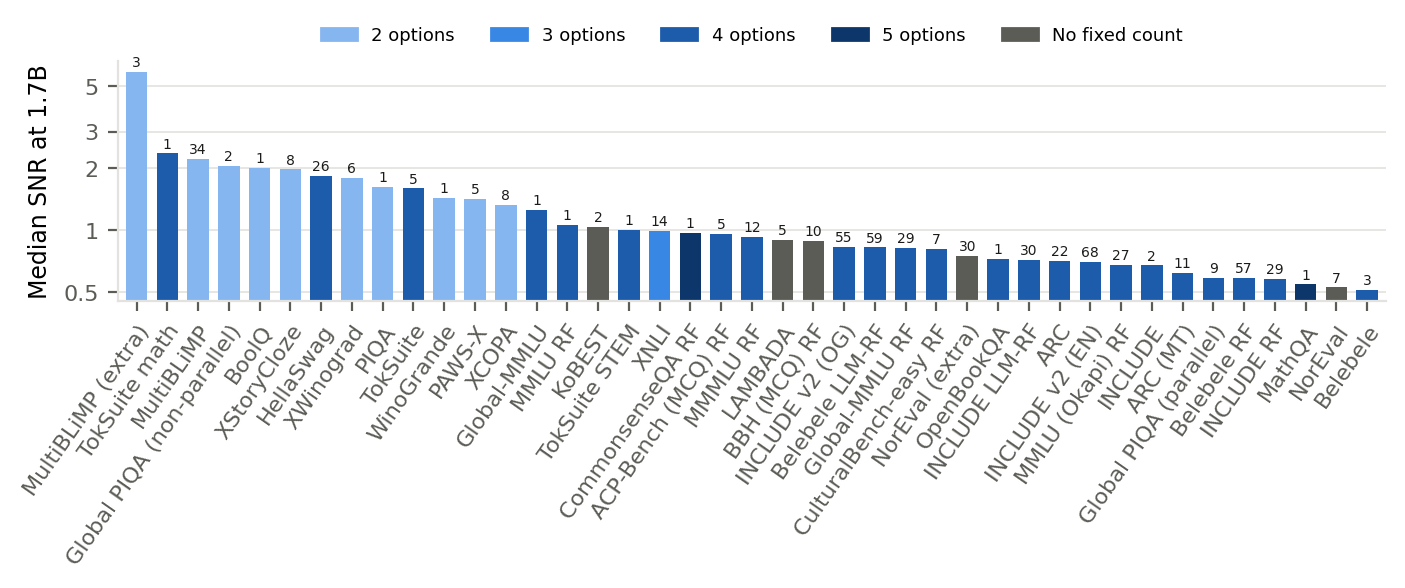
\includegraphics[width=\textwidth,height=0.36\textheight,keepaspectratio]{figures/app_rq09_benchmark_design.png}
% source: src/signal-and-noise/analysis/rq09_benchmark_design/pretraining/predictivity/snr_per_family_ranked_paper_horizontal.png
\captionof{figure}{\textbf{Among the families with at least five tasks, MultiBLiMP, HellaSwag and XStoryCloze separate the designs most sharply at 1.7B, and seven of the nine sharpest families have two answer options.} Median SNR at 1.7B over the per-language tasks of each benchmark family that clears the above-chance gate, ranked, on a log scale. The number above a bar counts its tasks. The colour gives the number of answer options (grey: LAMBADA scores a last word and BBH mixes two to eight).}
\label{fig:app_rq09_benchmark_design}
\end{minipage}
}]



\begin{figure*}[p]
\centering
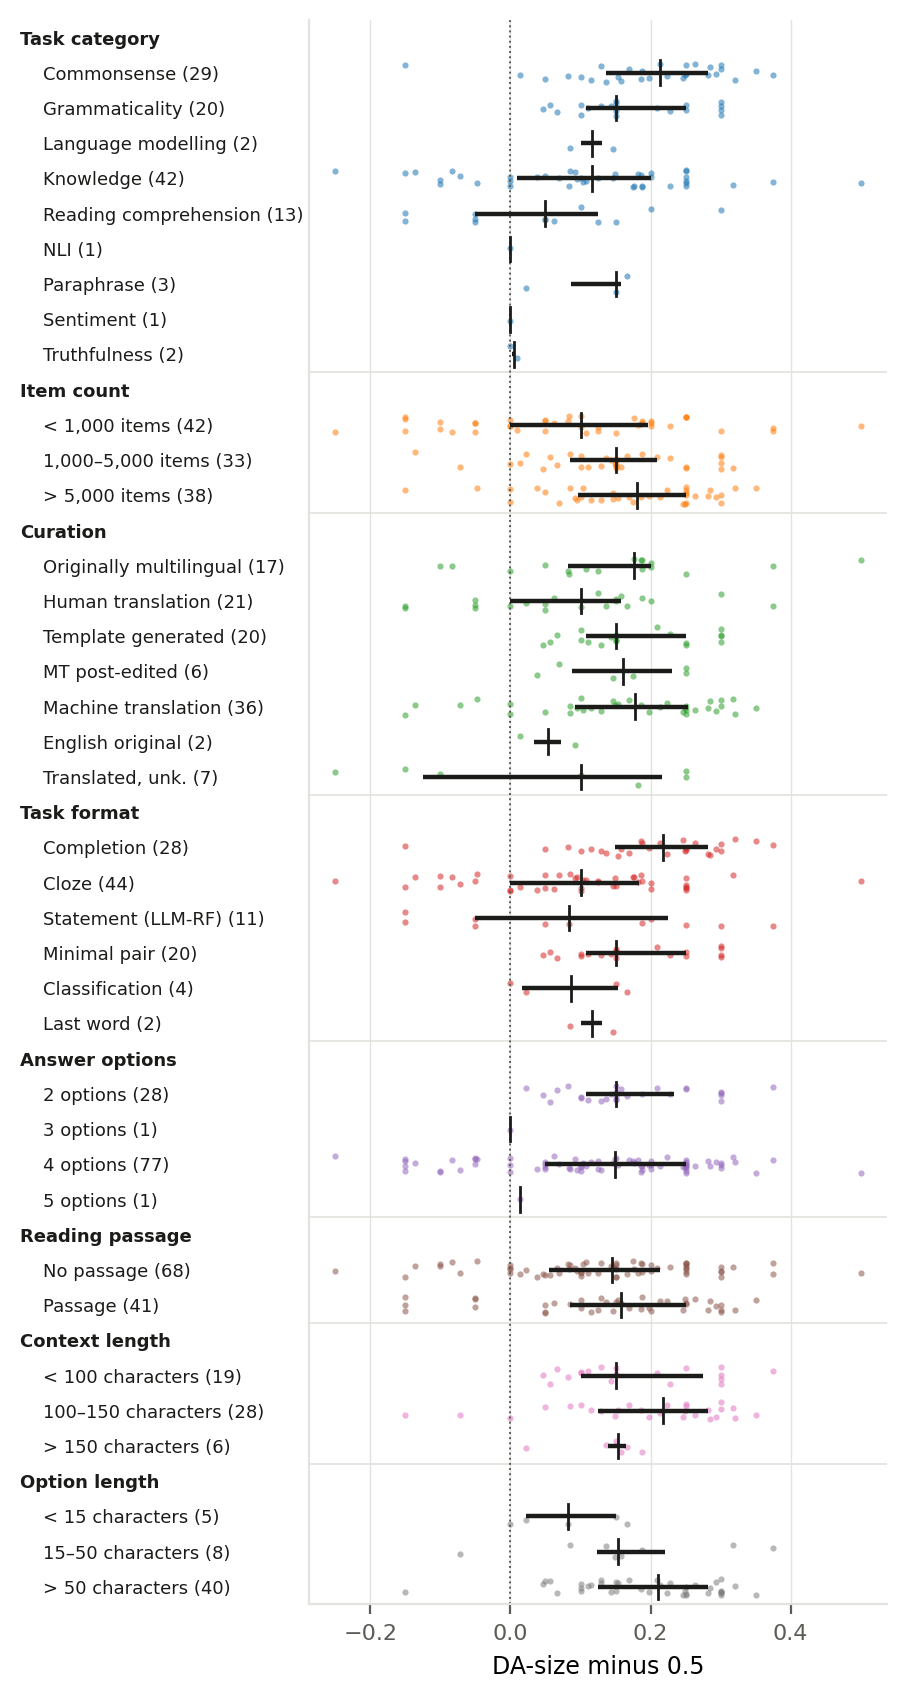
\includegraphics[width=\textwidth,height=0.8\textheight,keepaspectratio]{figures/app_rq09_design_da_by_level.png}
% source: src/signal-and-noise/analysis/rq09_benchmark_design/pretraining/predictivity/design_da_size_by_level_per_task_above_66_either_mono_axis_paper.png
\caption{\textbf{Read per task, the 113 reliable tasks sit above chance agreement (median DA-size 0.65), but the levels overlap: the medians of the levels with at least five tasks lie between 0.55 and 0.72.} English original holds 2 tasks (0.55). NLI holds 1 task (0.50). Language modelling holds 2 tasks (0.62). Paraphrase holds 3 tasks (0.65). Sentiment holds 1 task (0.50). Truthfulness holds 2 tasks (0.50). Classification holds 4 tasks (0.59). Last word holds 2 tasks (0.62). 3 options holds 1 task (0.50). 5 options holds 1 task (0.51). The task category is the domain of each task (a suite's subtask has its own). No task with lettered options passes the reliability filter, so every task format is a continuation format. Item count and the two lengths are read in three bins, and the lengths exist only for the original benchmarks with sampled items (53 tasks). Each block is one characteristic, a header row and then one row per level with the number of tasks at that level. A dot is one task (one benchmark in one language) at its DA-size minus 0.5, so the dotted line is chance agreement, and 93 of the 113 tasks sit to its right. The bar is the level's median and the horizontal line its interquartile range over the tasks. DA-size is the per-task DA-size of Figure~\ref{fig:rq2}: the final checkpoint of each proxy against the 1.7B final, on the mono-axis design pairs of the seed-1904 runs, on the tasks above chance at the proxy and at 1.7B, averaged over the proxies 90M--1B that have one, on the tasks of 22 benchmarks that pass the reliability filter of Figure~\ref{fig:rq2}. Figure~\ref{fig:app_rq09_design_da_correlation} gives the same characteristics as one correlation per benchmark.}
\label{fig:app_rq09_design_da_by_level}
\end{figure*}


\begin{figure*}[p]
\centering
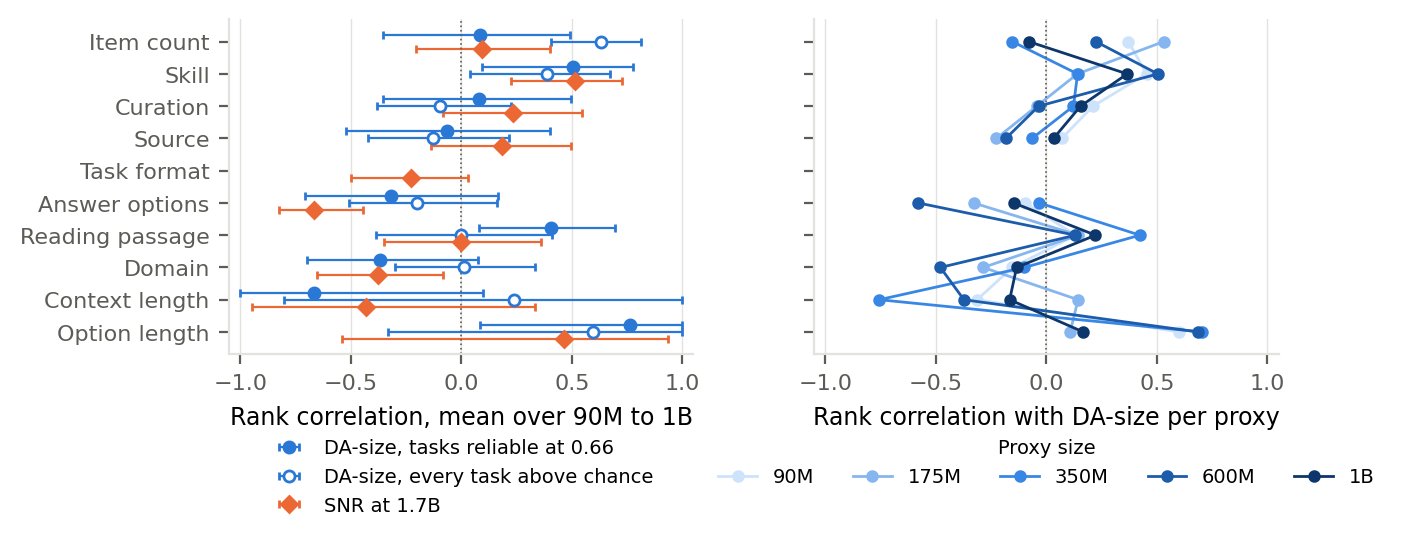
\includegraphics[width=\textwidth,height=0.8\textheight,keepaspectratio]{figures/app_rq09_design_da_correlation.png}
% source: src/signal-and-noise/analysis/rq09_benchmark_design/pretraining/predictivity/design_da_size_correlation_above_66_either_mono_axis_paper.png
\caption{\textbf{Item count orders the benchmarks by DA-size on every task above chance ($\rho = 0.63$) but not by SNR (0.10), and the LM-like skill correlates with both (0.39 and 0.51).} No other characteristic has a DA-size interval that excludes zero in both readings. The answer options, which correlate with SNR at $\rho = -0.67$ ($-0.82$ to $-0.44$), reach $-0.32$ on the reliable tasks and $-0.20$ on every task above chance. A row is one characteristic of the benchmark families (Table \ref{tab:app_rq09_benchmark_characteristics}). The value is a Spearman $\rho$ over the benchmarks against the characteristic's code: the options ranked 2 to 5, no passage to passage, and the item count (the median number of items over a benchmark's languages) and the two lengths as they are. Skill, curation, source, task format and domain are each split in two and coded from the first group to the second: knowledge, reading and reasoning to LM-like (commonsense, grammaticality and language modelling), translated to native (written in the language, English originals included, or generated from treebanks or planning problems), translated from English to not, continuation to lettered options, and the other domains to knowledge, the most common domain. A split whose smaller side holds one benchmark has no value, so task format has none on DA-size, where INCLUDE is the only benchmark with lettered options. A characteristic marked unknown in the table leaves that benchmark out of its row, except the curation of BBH, which was written in English and so counts as native. DA-size is the per-task DA-size of Figure~\ref{fig:rq2}: the final checkpoint of each proxy against the 1.7B final, on the mono-axis design pairs of the seed-1904 runs, on the tasks above chance at the proxy and at 1.7B. A benchmark's DA-size is the median over its tasks at a proxy, averaged over the proxies 90M--1B at which it has a task. Left: that mean with a 95\% bootstrap interval over the 22 benchmarks whose tasks pass the reliability filter of Figure~\ref{fig:rq2} (filled), over the 39 benchmarks with any task above chance (hollow), and the same statistics on the median SNR at 1.7B of the 41 benchmarks (diamonds). Right: one line per proxy size, on the reliable tasks, over 17 to 22 benchmarks per proxy. The lengths exist for the original benchmarks with sampled items only.}
\label{fig:app_rq09_design_da_correlation}
\end{figure*}

\begin{table*}[p]
\centering
\small
\begin{adjustbox}{max width=\textwidth}
\begin{tabular}{llllllrrr}
\toprule
Benchmark & Domain & Curation & Source & Format & Options & Passage & Context & Option \\
\midrule
ACP-Bench (MCQ) RF & reasoning & template & English & cloze & 4 & yes & -- & -- \\
ARC & knowledge & MT & translated & cloze & 4 & no & 122 & 28 \\
ARC (MT) & knowledge & MT & translated & cloze & 4 & no & -- & -- \\
BBH (MCQ) RF & reasoning & unknown & English & cloze & 2--8 & unknown & -- & -- \\
Belebele & reading comprehension & human transl. & translated & MCQ + passage & 4 & yes & 558 & 21 \\
Belebele LLM-RF & reading comprehension & human transl. & translated & statement (LLM-RF) & 4 & yes & -- & -- \\
Belebele RF & reading comprehension & human transl. & translated & cloze & 4 & yes & -- & -- \\
CommonsenseQA RF & commonsense & English & English & cloze & 5 & no & -- & -- \\
CulturalBench-easy RF & culture & English & English & cloze & 4 & no & -- & -- \\
Global PIQA (non-parallel) & commonsense & native & native & completion & 2 & no & -- & -- \\
Global PIQA (parallel) & commonsense & MT + post-edit & translated & completion & 4 & no & -- & -- \\
Global-MMLU & knowledge & MT + post-edit & translated & MCQ & 4 & no & 120 & 11 \\
Global-MMLU RF & knowledge & MT + post-edit & translated & cloze & 4 & no & -- & -- \\
HellaSwag & commonsense & MT & translated & completion & 4 & yes & 118 & 61 \\
INCLUDE & knowledge & native & native & MCQ & 4 & no & -- & -- \\
INCLUDE LLM-RF & knowledge & native & native & statement (LLM-RF) & 4 & no & -- & -- \\
INCLUDE RF & knowledge & native & native & cloze & 4 & no & -- & -- \\
INCLUDE v2 (EN) & knowledge & transl. (unknown) & native & cloze & 4 & no & -- & -- \\
INCLUDE v2 (OG) & knowledge & native & native & cloze & 4 & no & -- & -- \\
LAMBADA & language modelling & MT & translated & last word & -- & yes & -- & -- \\
MMLU RF & knowledge & English & English & cloze & 4 & no & -- & -- \\
MathQA & math & English & English & cloze & 5 & no & -- & -- \\
MultiBLiMP & grammaticality & template & native & minimal pair & 2 & no & 46 & 119 \\
OpenBookQA & knowledge & English & English & completion & 4 & no & -- & -- \\
PAWS-X & paraphrase & human transl. & translated & classification & 2 & no & 224 & 2 \\
XCOPA & commonsense & human transl. & translated & completion & 2 & no & 37 & 31 \\
XNLI & NLI & human transl. & translated & classification & 3 & no & 127 & 10 \\
XStoryCloze & commonsense & human transl. & translated & completion & 2 & yes & 189 & 38 \\
XWinograd & commonsense & native & native & completion & 2 & no & 74 & 6 \\
\bottomrule
\end{tabular}

\end{adjustbox}
% source: src/signal-and-noise/analysis/rq09_benchmark_design/pretraining/predictivity/benchmark_characteristics.tex
\caption{\textbf{The 41 benchmark families of the benchmark design analysis and the characteristics it groups them by.} 17 are translated from English, 12 are English originals evaluated in English, and 23 have four answer options. Domain: what the benchmark tests, as its own paper describes it (15 test knowledge, the domain the analysis contrasts with the rest). Curation: how the items in each language were made (native: written in the language, English: written in English, human transl.: translated by people, MT: machine translated, MT + post-edit: machine translated and corrected, transl. (unknown): translated by a method the dataset does not document, template: generated from treebank or planning templates). Source: whether the benchmark was translated from English, written natively in several languages or written in English. Format (as the evaluation prompts it): MCQ is a question with lettered options, cloze scores each option as a continuation of the question, completion scores continuations of a context, statement (LLM-RF) is the LLM rewrite into a statement with four continuations, last word scores the final word of a passage. Options gives the range where subtasks differ. Unknown marks a characteristic no source settles, which the analysis leaves out, except the curation of BBH, which counts as native because its items were written in English. Mixed marks a suite whose subtasks differ, which the analysis also leaves out. Skill groups the domains: LM-like for commonsense, grammaticality and language modelling (12 benchmarks), knowledge etc. for the rest. Items: the median number of items over the benchmark's languages. Context and Option: the median characters of the context and of an option over 100 sampled English items.}
\label{tab:app_rq09_benchmark_characteristics}
\end{table*}
